\documentclass{standalone}
\usepackage{tikz}
\usetikzlibrary{patterns, positioning}


\begin{document}
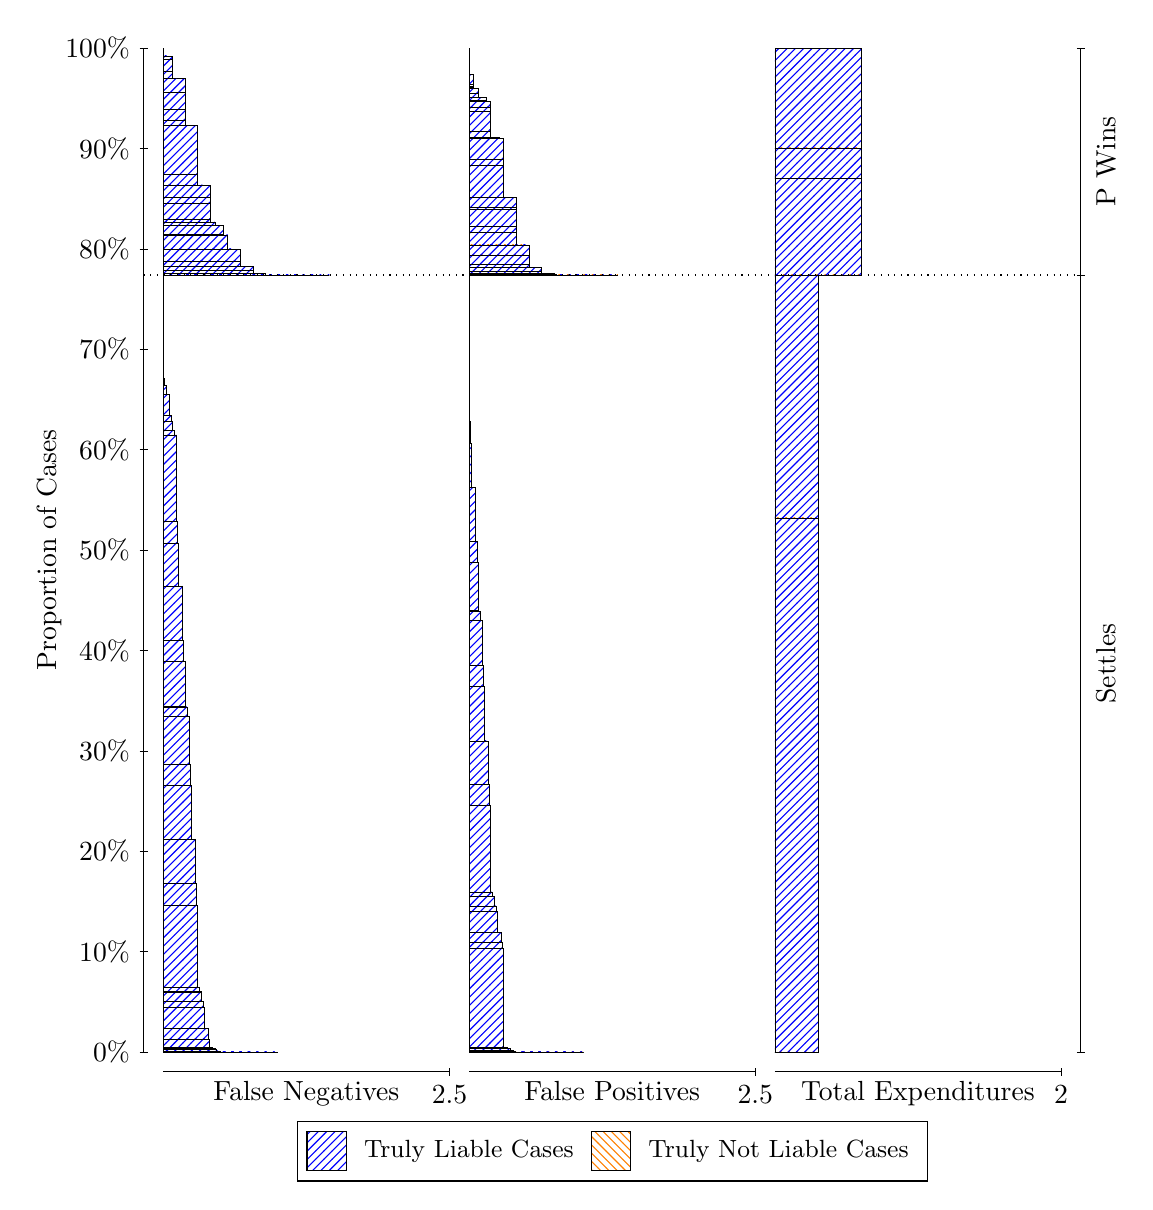
\begin{tikzpicture}
\draw[black, very thin] (1.5,1.75) -- (1.5,14.5);
\node[rotate=90, text=black, anchor=center] at (0.3, 8.125) {Proportion of Cases};
\draw[black, very thin] (1.45,1.75) -- (1.55,1.75);
\node[text=black, anchor=east] at (1.45, 1.75) {0\%};
\draw[black, very thin] (1.45,3.025) -- (1.55,3.025);
\node[text=black, anchor=east] at (1.45, 3.025) {10\%};
\draw[black, very thin] (1.45,4.3) -- (1.55,4.3);
\node[text=black, anchor=east] at (1.45, 4.3) {20\%};
\draw[black, very thin] (1.45,5.575) -- (1.55,5.575);
\node[text=black, anchor=east] at (1.45, 5.575) {30\%};
\draw[black, very thin] (1.45,6.85) -- (1.55,6.85);
\node[text=black, anchor=east] at (1.45, 6.85) {40\%};
\draw[black, very thin] (1.45,8.125) -- (1.55,8.125);
\node[text=black, anchor=east] at (1.45, 8.125) {50\%};
\draw[black, very thin] (1.45,9.4) -- (1.55,9.4);
\node[text=black, anchor=east] at (1.45, 9.4) {60\%};
\draw[black, very thin] (1.45,10.675) -- (1.55,10.675);
\node[text=black, anchor=east] at (1.45, 10.675) {70\%};
\draw[black, very thin] (1.45,11.95) -- (1.55,11.95);
\node[text=black, anchor=east] at (1.45, 11.95) {80\%};
\draw[black, very thin] (1.45,13.225) -- (1.55,13.225);
\node[text=black, anchor=east] at (1.45, 13.225) {90\%};
\draw[black, very thin] (1.45,14.5) -- (1.55,14.5);
\node[text=black, anchor=east] at (1.45, 14.5) {100\%};

\draw[black, very thin] (13.4,1.75) -- (13.4,14.5);
\draw[black, very thin] (13.35,1.75) -- (13.45,1.75);
\node[anchor=west] at (13.35, 1.75) {};
\draw[black, very thin] (13.35,11.618) -- (13.45,11.618);
\node[anchor=west] at (13.35, 11.618) {};
\draw[black, very thin] (13.35,14.5) -- (13.45,14.5);
\node[anchor=west] at (13.35, 14.5) {};

\draw[black, very thin, pattern color=blue, pattern=north east lines] (1.75,1.75) rectangle (3.2033,1.75);
\draw[black, very thin, pattern color=blue, pattern=north east lines] (1.75,1.75) rectangle (3.058,1.75);
\draw[black, very thin, pattern color=blue, pattern=north east lines] (1.75,1.75) rectangle (3.0419,1.75);
\draw[black, very thin, pattern color=blue, pattern=north east lines] (1.75,1.75) rectangle (2.9127,1.75);
\draw[black, very thin, pattern color=blue, pattern=north east lines] (1.75,1.75) rectangle (2.8965,1.75);
\draw[black, very thin, pattern color=blue, pattern=north east lines] (1.75,1.75) rectangle (2.8804,1.75);
\draw[black, very thin, pattern color=blue, pattern=north east lines] (1.75,1.75) rectangle (2.84,1.75);
\draw[black, very thin, pattern color=blue, pattern=north east lines] (1.75,1.75) rectangle (2.7512,1.75);
\draw[black, very thin, pattern color=blue, pattern=north east lines] (1.75,1.75) rectangle (2.735,1.75);
\draw[black, very thin, pattern color=blue, pattern=north east lines] (1.75,1.75) rectangle (2.7189,1.75);
\draw[black, very thin, pattern color=blue, pattern=north east lines] (1.75,1.75) rectangle (2.6947,1.75);
\draw[black, very thin, pattern color=blue, pattern=north east lines] (1.75,1.75) rectangle (2.6785,1.75);
\draw[black, very thin, pattern color=blue, pattern=north east lines] (1.75,1.75) rectangle (2.5897,1.7505);
\draw[black, very thin, pattern color=blue, pattern=north east lines] (1.75,1.7505) rectangle (2.5736,1.7506);
\draw[black, very thin, pattern color=blue, pattern=north east lines] (1.75,1.7506) rectangle (2.5574,1.7507);
\draw[black, very thin, pattern color=blue, pattern=north east lines] (1.75,1.7507) rectangle (2.5493,1.7507);
\draw[black, very thin, pattern color=blue, pattern=north east lines] (1.75,1.7507) rectangle (2.5332,1.7508);
\draw[black, very thin, pattern color=blue, pattern=north east lines] (1.75,1.7508) rectangle (2.517,1.7508);
\draw[black, very thin, pattern color=blue, pattern=north east lines] (1.75,1.7508) rectangle (2.4767,1.7627);
\draw[black, very thin, pattern color=blue, pattern=north east lines] (1.75,1.7627) rectangle (2.4282,1.7888);
\draw[black, very thin, pattern color=blue, pattern=north east lines] (1.75,1.7888) rectangle (2.4121,1.7943);
\draw[black, very thin, pattern color=blue, pattern=north east lines] (1.75,1.7943) rectangle (2.3959,1.7999);
\draw[black, very thin, pattern color=blue, pattern=north east lines] (1.75,1.7999) rectangle (2.3879,1.8002);
\draw[black, very thin, pattern color=blue, pattern=north east lines] (1.75,1.8002) rectangle (2.3717,1.8052);
\draw[black, very thin, pattern color=blue, pattern=north east lines] (1.75,1.8052) rectangle (2.3556,1.8054);
\draw[black, very thin, pattern color=blue, pattern=north east lines] (1.75,1.8054) rectangle (2.3313,1.9166);
\draw[black, very thin, pattern color=blue, pattern=north east lines] (1.75,1.9166) rectangle (2.3152,2.0531);
\draw[black, very thin, pattern color=blue, pattern=north east lines] (1.75,2.0531) rectangle (2.2667,2.3172);
\draw[black, very thin, pattern color=blue, pattern=north east lines] (1.75,2.3172) rectangle (2.2506,2.391);
\draw[black, very thin, pattern color=blue, pattern=north east lines] (1.75,2.391) rectangle (2.2344,2.5123);
\draw[black, very thin, pattern color=blue, pattern=north east lines] (1.75,2.5123) rectangle (2.2264,2.5147);
\draw[black, very thin, pattern color=blue, pattern=north east lines] (1.75,2.5147) rectangle (2.2102,2.5678);
\draw[black, very thin, pattern color=blue, pattern=north east lines] (1.75,2.5678) rectangle (2.1941,2.5702);
\draw[black, very thin, pattern color=blue, pattern=north east lines] (1.75,2.5702) rectangle (2.186,3.6107);
\draw[black, very thin, pattern color=blue, pattern=north east lines] (1.75,3.6107) rectangle (2.1699,3.8927);
\draw[black, very thin, pattern color=blue, pattern=north east lines] (1.75,3.8927) rectangle (2.1537,4.4453);
\draw[black, very thin, pattern color=blue, pattern=north east lines] (1.75,4.4453) rectangle (2.1053,5.1353);
\draw[black, very thin, pattern color=blue, pattern=north east lines] (1.75,5.1353) rectangle (2.0891,5.4048);
\draw[black, very thin, pattern color=blue, pattern=north east lines] (1.75,5.4048) rectangle (2.073,6.011);
\draw[black, very thin, pattern color=blue, pattern=north east lines] (1.75,6.011) rectangle (2.0649,6.0167);
\draw[black, very thin, pattern color=blue, pattern=north east lines] (1.75,6.0167) rectangle (2.0487,6.1333);
\draw[black, very thin, pattern color=blue, pattern=north east lines] (1.75,6.1333) rectangle (2.0326,6.1389);
\draw[black, very thin, pattern color=blue, pattern=north east lines] (1.75,6.1389) rectangle (2.0245,6.7102);
\draw[black, very thin, pattern color=blue, pattern=north east lines] (1.75,6.7102) rectangle (2.0084,6.9777);
\draw[black, very thin, pattern color=blue, pattern=north east lines] (1.75,6.9777) rectangle (1.9922,7.668);
\draw[black, very thin, pattern color=blue, pattern=north east lines] (1.75,7.668) rectangle (1.9438,8.214);
\draw[black, very thin, pattern color=blue, pattern=north east lines] (1.75,8.214) rectangle (1.9276,8.4868);
\draw[black, very thin, pattern color=blue, pattern=north east lines] (1.75,8.4868) rectangle (1.9115,9.5858);
\draw[black, very thin, pattern color=blue, pattern=north east lines] (1.75,9.5858) rectangle (1.9034,9.5882);
\draw[black, very thin, pattern color=blue, pattern=north east lines] (1.75,9.5882) rectangle (1.8873,9.6412);
\draw[black, very thin, pattern color=blue, pattern=north east lines] (1.75,9.6412) rectangle (1.8711,9.6436);
\draw[black, very thin, pattern color=blue, pattern=north east lines] (1.75,9.6436) rectangle (1.863,9.7616);
\draw[black, very thin, pattern color=blue, pattern=north east lines] (1.75,9.7616) rectangle (1.8469,9.8352);
\draw[black, very thin, pattern color=blue, pattern=north east lines] (1.75,9.8352) rectangle (1.8307,10.099);
\draw[black, very thin, pattern color=blue, pattern=north east lines] (1.75,10.099) rectangle (1.7823,10.22);
\draw[black, very thin, pattern color=blue, pattern=north east lines] (1.75,10.22) rectangle (1.7661,10.304);
\draw[black, very thin, pattern color=orange, pattern=north west lines] (1.75,10.304) rectangle (1.75,10.304);
\draw[black, very thin, pattern color=blue, pattern=north east lines] (1.75,10.304) rectangle (1.75,11.618);
\draw[black, very thin, pattern color=blue, pattern=north east lines] (1.75,11.618) rectangle (3.8573,11.618);
\draw[black, very thin, pattern color=blue, pattern=north east lines] (1.75,11.618) rectangle (3.6959,11.618);
\draw[black, very thin, pattern color=blue, pattern=north east lines] (1.75,11.618) rectangle (3.5344,11.618);
\draw[black, very thin, pattern color=blue, pattern=north east lines] (1.75,11.618) rectangle (3.5344,11.618);
\draw[black, very thin, pattern color=blue, pattern=north east lines] (1.75,11.618) rectangle (3.3729,11.618);
\draw[black, very thin, pattern color=blue, pattern=north east lines] (1.75,11.618) rectangle (3.3164,11.618);
\draw[black, very thin, pattern color=blue, pattern=north east lines] (1.75,11.618) rectangle (3.2114,11.62);
\draw[black, very thin, pattern color=blue, pattern=north east lines] (1.75,11.62) rectangle (3.1549,11.62);
\draw[black, very thin, pattern color=blue, pattern=north east lines] (1.75,11.62) rectangle (3.1549,11.62);
\draw[black, very thin, pattern color=blue, pattern=north east lines] (1.75,11.62) rectangle (3.0499,11.64);
\draw[black, very thin, pattern color=blue, pattern=north east lines] (1.75,11.64) rectangle (2.9934,11.64);
\draw[black, very thin, pattern color=blue, pattern=north east lines] (1.75,11.64) rectangle (2.9934,11.64);
\draw[black, very thin, pattern color=blue, pattern=north east lines] (1.75,11.64) rectangle (2.8884,11.673);
\draw[black, very thin, pattern color=blue, pattern=north east lines] (1.75,11.673) rectangle (2.8884,11.73);
\draw[black, very thin, pattern color=blue, pattern=north east lines] (1.75,11.73) rectangle (2.8319,11.73);
\draw[black, very thin, pattern color=blue, pattern=north east lines] (1.75,11.73) rectangle (2.727,11.797);
\draw[black, very thin, pattern color=blue, pattern=north east lines] (1.75,11.797) rectangle (2.727,11.939);
\draw[black, very thin, pattern color=blue, pattern=north east lines] (1.75,11.939) rectangle (2.6704,11.949);
\draw[black, very thin, pattern color=blue, pattern=north east lines] (1.75,11.949) rectangle (2.5655,12.117);
\draw[black, very thin, pattern color=blue, pattern=north east lines] (1.75,12.117) rectangle (2.5655,12.128);
\draw[black, very thin, pattern color=blue, pattern=north east lines] (1.75,12.128) rectangle (2.509,12.129);
\draw[black, very thin, pattern color=blue, pattern=north east lines] (1.75,12.129) rectangle (2.509,12.246);
\draw[black, very thin, pattern color=blue, pattern=north east lines] (1.75,12.246) rectangle (2.404,12.293);
\draw[black, very thin, pattern color=blue, pattern=north east lines] (1.75,12.293) rectangle (2.3475,12.331);
\draw[black, very thin, pattern color=blue, pattern=north east lines] (1.75,12.331) rectangle (2.3475,12.533);
\draw[black, very thin, pattern color=blue, pattern=north east lines] (1.75,12.533) rectangle (2.3475,12.607);
\draw[black, very thin, pattern color=blue, pattern=north east lines] (1.75,12.607) rectangle (2.3475,12.757);
\draw[black, very thin, pattern color=blue, pattern=north east lines] (1.75,12.757) rectangle (2.2425,12.761);
\draw[black, very thin, pattern color=blue, pattern=north east lines] (1.75,12.761) rectangle (2.2425,12.761);
\draw[black, very thin, pattern color=blue, pattern=north east lines] (1.75,12.761) rectangle (2.186,12.896);
\draw[black, very thin, pattern color=blue, pattern=north east lines] (1.75,12.896) rectangle (2.186,13.513);
\draw[black, very thin, pattern color=blue, pattern=north east lines] (1.75,13.513) rectangle (2.081,13.513);
\draw[black, very thin, pattern color=blue, pattern=north east lines] (1.75,13.513) rectangle (2.081,13.513);
\draw[black, very thin, pattern color=blue, pattern=north east lines] (1.75,13.513) rectangle (2.0245,13.586);
\draw[black, very thin, pattern color=blue, pattern=north east lines] (1.75,13.586) rectangle (2.0245,13.716);
\draw[black, very thin, pattern color=blue, pattern=north east lines] (1.75,13.716) rectangle (2.0245,13.939);
\draw[black, very thin, pattern color=blue, pattern=north east lines] (1.75,13.939) rectangle (2.0245,14.117);
\draw[black, very thin, pattern color=blue, pattern=north east lines] (1.75,14.117) rectangle (1.9196,14.117);
\draw[black, very thin, pattern color=blue, pattern=north east lines] (1.75,14.117) rectangle (1.9196,14.117);
\draw[black, very thin, pattern color=blue, pattern=north east lines] (1.75,14.117) rectangle (1.863,14.203);
\draw[black, very thin, pattern color=blue, pattern=north east lines] (1.75,14.203) rectangle (1.863,14.363);
\draw[black, very thin, pattern color=blue, pattern=north east lines] (1.75,14.363) rectangle (1.863,14.4);
\draw[black, very thin, pattern color=blue, pattern=north east lines] (1.75,14.4) rectangle (1.7581,14.4);
\draw[black, very thin, pattern color=blue, pattern=north east lines] (1.75,14.4) rectangle (1.7581,14.4);
\draw[black, very thin, pattern color=orange, pattern=north west lines] (1.75,14.4) rectangle (1.75,14.4);
\draw[black, very thin, pattern color=blue, pattern=north east lines] (1.75,14.4) rectangle (1.75,14.5);
\draw[black, very thin, pattern color=orange, pattern=north west lines] (5.6333,1.75) rectangle (7.0867,1.75);
\draw[black, very thin, pattern color=blue, pattern=north east lines] (5.6333,1.75) rectangle (7.0867,1.75);
\draw[black, very thin, pattern color=orange, pattern=north west lines] (5.6333,1.75) rectangle (6.9413,1.75);
\draw[black, very thin, pattern color=blue, pattern=north east lines] (5.6333,1.75) rectangle (6.9413,1.75);
\draw[black, very thin, pattern color=blue, pattern=north east lines] (5.6333,1.75) rectangle (6.9252,1.75);
\draw[black, very thin, pattern color=orange, pattern=north west lines] (5.6333,1.75) rectangle (6.796,1.75);
\draw[black, very thin, pattern color=blue, pattern=north east lines] (5.6333,1.75) rectangle (6.796,1.75);
\draw[black, very thin, pattern color=blue, pattern=north east lines] (5.6333,1.75) rectangle (6.7799,1.75);
\draw[black, very thin, pattern color=blue, pattern=north east lines] (5.6333,1.75) rectangle (6.7637,1.75);
\draw[black, very thin, pattern color=orange, pattern=north west lines] (5.6333,1.75) rectangle (6.7233,1.75);
\draw[black, very thin, pattern color=blue, pattern=north east lines] (5.6333,1.75) rectangle (6.7233,1.75);
\draw[black, very thin, pattern color=blue, pattern=north east lines] (5.6333,1.75) rectangle (6.6345,1.75);
\draw[black, very thin, pattern color=blue, pattern=north east lines] (5.6333,1.75) rectangle (6.6184,1.75);
\draw[black, very thin, pattern color=blue, pattern=north east lines] (5.6333,1.75) rectangle (6.6022,1.75);
\draw[black, very thin, pattern color=orange, pattern=north west lines] (5.6333,1.75) rectangle (6.578,1.75);
\draw[black, very thin, pattern color=blue, pattern=north east lines] (5.6333,1.75) rectangle (6.578,1.75);
\draw[black, very thin, pattern color=blue, pattern=north east lines] (5.6333,1.75) rectangle (6.5619,1.75);
\draw[black, very thin, pattern color=blue, pattern=north east lines] (5.6333,1.75) rectangle (6.473,1.75);
\draw[black, very thin, pattern color=blue, pattern=north east lines] (5.6333,1.75) rectangle (6.4569,1.75);
\draw[black, very thin, pattern color=blue, pattern=north east lines] (5.6333,1.75) rectangle (6.4407,1.75);
\draw[black, very thin, pattern color=orange, pattern=north west lines] (5.6333,1.75) rectangle (6.4327,1.75);
\draw[black, very thin, pattern color=blue, pattern=north east lines] (5.6333,1.75) rectangle (6.4327,1.75);
\draw[black, very thin, pattern color=blue, pattern=north east lines] (5.6333,1.75) rectangle (6.4165,1.75);
\draw[black, very thin, pattern color=blue, pattern=north east lines] (5.6333,1.75) rectangle (6.4004,1.75);
\draw[black, very thin, pattern color=orange, pattern=north west lines] (5.6333,1.75) rectangle (6.36,1.75);
\draw[black, very thin, pattern color=blue, pattern=north east lines] (5.6333,1.75) rectangle (6.36,1.7501);
\draw[black, very thin, pattern color=blue, pattern=north east lines] (5.6333,1.7501) rectangle (6.3116,1.7506);
\draw[black, very thin, pattern color=blue, pattern=north east lines] (5.6333,1.7506) rectangle (6.2954,1.7507);
\draw[black, very thin, pattern color=blue, pattern=north east lines] (5.6333,1.7507) rectangle (6.2793,1.7508);
\draw[black, very thin, pattern color=blue, pattern=north east lines] (5.6333,1.7508) rectangle (6.2712,1.7508);
\draw[black, very thin, pattern color=blue, pattern=north east lines] (5.6333,1.7508) rectangle (6.255,1.7509);
\draw[black, very thin, pattern color=blue, pattern=north east lines] (5.6333,1.7509) rectangle (6.2389,1.7509);
\draw[black, very thin, pattern color=orange, pattern=north west lines] (5.6333,1.7509) rectangle (6.2147,1.7509);
\draw[black, very thin, pattern color=blue, pattern=north east lines] (5.6333,1.7509) rectangle (6.2147,1.7622);
\draw[black, very thin, pattern color=blue, pattern=north east lines] (5.6333,1.7622) rectangle (6.1985,1.7687);
\draw[black, very thin, pattern color=blue, pattern=north east lines] (5.6333,1.7687) rectangle (6.1501,1.7949);
\draw[black, very thin, pattern color=blue, pattern=north east lines] (5.6333,1.7949) rectangle (6.1339,1.8003);
\draw[black, very thin, pattern color=blue, pattern=north east lines] (5.6333,1.8003) rectangle (6.1178,1.806);
\draw[black, very thin, pattern color=blue, pattern=north east lines] (5.6333,1.806) rectangle (6.1097,1.8062);
\draw[black, very thin, pattern color=blue, pattern=north east lines] (5.6333,1.8062) rectangle (6.0936,1.8111);
\draw[black, very thin, pattern color=blue, pattern=north east lines] (5.6333,1.8111) rectangle (6.0774,1.8113);
\draw[black, very thin, pattern color=orange, pattern=north west lines] (5.6333,1.8113) rectangle (6.0693,1.8113);
\draw[black, very thin, pattern color=blue, pattern=north east lines] (5.6333,1.8113) rectangle (6.0693,3.0635);
\draw[black, very thin, pattern color=blue, pattern=north east lines] (5.6333,3.0635) rectangle (6.0532,3.1482);
\draw[black, very thin, pattern color=blue, pattern=north east lines] (5.6333,3.1482) rectangle (6.037,3.2686);
\draw[black, very thin, pattern color=blue, pattern=north east lines] (5.6333,3.2686) rectangle (5.9886,3.5327);
\draw[black, very thin, pattern color=blue, pattern=north east lines] (5.6333,3.5327) rectangle (5.9724,3.6063);
\draw[black, very thin, pattern color=blue, pattern=north east lines] (5.6333,3.6063) rectangle (5.9563,3.7243);
\draw[black, very thin, pattern color=blue, pattern=north east lines] (5.6333,3.7243) rectangle (5.9482,3.7267);
\draw[black, very thin, pattern color=blue, pattern=north east lines] (5.6333,3.7267) rectangle (5.9321,3.7798);
\draw[black, very thin, pattern color=blue, pattern=north east lines] (5.6333,3.7798) rectangle (5.9159,3.7822);
\draw[black, very thin, pattern color=blue, pattern=north east lines] (5.6333,3.7822) rectangle (5.9079,4.8812);
\draw[black, very thin, pattern color=blue, pattern=north east lines] (5.6333,4.8812) rectangle (5.8917,5.1539);
\draw[black, very thin, pattern color=blue, pattern=north east lines] (5.6333,5.1539) rectangle (5.8756,5.6999);
\draw[black, very thin, pattern color=blue, pattern=north east lines] (5.6333,5.6999) rectangle (5.8271,6.3903);
\draw[black, very thin, pattern color=blue, pattern=north east lines] (5.6333,6.3903) rectangle (5.811,6.6577);
\draw[black, very thin, pattern color=blue, pattern=north east lines] (5.6333,6.6577) rectangle (5.7948,7.229);
\draw[black, very thin, pattern color=blue, pattern=north east lines] (5.6333,7.229) rectangle (5.7867,7.2347);
\draw[black, very thin, pattern color=blue, pattern=north east lines] (5.6333,7.2347) rectangle (5.7706,7.3513);
\draw[black, very thin, pattern color=blue, pattern=north east lines] (5.6333,7.3513) rectangle (5.7544,7.3569);
\draw[black, very thin, pattern color=blue, pattern=north east lines] (5.6333,7.3569) rectangle (5.7464,7.9631);
\draw[black, very thin, pattern color=blue, pattern=north east lines] (5.6333,7.9631) rectangle (5.7302,8.2326);
\draw[black, very thin, pattern color=blue, pattern=north east lines] (5.6333,8.2326) rectangle (5.7141,8.9226);
\draw[black, very thin, pattern color=blue, pattern=north east lines] (5.6333,8.9226) rectangle (5.6656,9.4752);
\draw[black, very thin, pattern color=blue, pattern=north east lines] (5.6333,9.4752) rectangle (5.6495,9.7572);
\draw[black, very thin, pattern color=blue, pattern=north east lines] (5.6333,9.7572) rectangle (5.6333,11.618);
\draw[black, very thin, pattern color=orange, pattern=north west lines] (5.6333,11.618) rectangle (7.5227,11.618);
\draw[black, very thin, pattern color=blue, pattern=north east lines] (5.6333,11.618) rectangle (7.5227,11.618);
\draw[black, very thin, pattern color=orange, pattern=north west lines] (5.6333,11.618) rectangle (7.3612,11.618);
\draw[black, very thin, pattern color=blue, pattern=north east lines] (5.6333,11.618) rectangle (7.3612,11.618);
\draw[black, very thin, pattern color=blue, pattern=north east lines] (5.6333,11.618) rectangle (7.1997,11.618);
\draw[black, very thin, pattern color=orange, pattern=north west lines] (5.6333,11.618) rectangle (7.1997,11.618);
\draw[black, very thin, pattern color=blue, pattern=north east lines] (5.6333,11.618) rectangle (7.1997,11.618);
\draw[black, very thin, pattern color=blue, pattern=north east lines] (5.6333,11.618) rectangle (7.0382,11.618);
\draw[black, very thin, pattern color=blue, pattern=north east lines] (5.6333,11.618) rectangle (7.0382,11.618);
\draw[black, very thin, pattern color=orange, pattern=north west lines] (5.6333,11.618) rectangle (7.0382,11.618);
\draw[black, very thin, pattern color=blue, pattern=north east lines] (5.6333,11.618) rectangle (7.0382,11.618);
\draw[black, very thin, pattern color=orange, pattern=north west lines] (5.6333,11.618) rectangle (6.8767,11.618);
\draw[black, very thin, pattern color=blue, pattern=north east lines] (5.6333,11.618) rectangle (6.8767,11.619);
\draw[black, very thin, pattern color=blue, pattern=north east lines] (5.6333,11.619) rectangle (6.8767,11.619);
\draw[black, very thin, pattern color=blue, pattern=north east lines] (5.6333,11.619) rectangle (6.8767,11.619);
\draw[black, very thin, pattern color=orange, pattern=north west lines] (5.6333,11.619) rectangle (6.7153,11.619);
\draw[black, very thin, pattern color=blue, pattern=north east lines] (5.6333,11.619) rectangle (6.7153,11.632);
\draw[black, very thin, pattern color=blue, pattern=north east lines] (5.6333,11.632) rectangle (6.7153,11.634);
\draw[black, very thin, pattern color=orange, pattern=north west lines] (5.6333,11.634) rectangle (6.6587,11.634);
\draw[black, very thin, pattern color=blue, pattern=north east lines] (5.6333,11.634) rectangle (6.6587,11.634);
\draw[black, very thin, pattern color=blue, pattern=north east lines] (5.6333,11.634) rectangle (6.5538,11.662);
\draw[black, very thin, pattern color=orange, pattern=north west lines] (5.6333,11.662) rectangle (6.5538,11.662);
\draw[black, very thin, pattern color=blue, pattern=north east lines] (5.6333,11.662) rectangle (6.5538,11.718);
\draw[black, very thin, pattern color=blue, pattern=north east lines] (5.6333,11.718) rectangle (6.4973,11.718);
\draw[black, very thin, pattern color=orange, pattern=north west lines] (5.6333,11.718) rectangle (6.4973,11.718);
\draw[black, very thin, pattern color=blue, pattern=north east lines] (5.6333,11.718) rectangle (6.4973,11.718);
\draw[black, very thin, pattern color=blue, pattern=north east lines] (5.6333,11.718) rectangle (6.3923,11.755);
\draw[black, very thin, pattern color=blue, pattern=north east lines] (5.6333,11.755) rectangle (6.3923,11.873);
\draw[black, very thin, pattern color=orange, pattern=north west lines] (5.6333,11.873) rectangle (6.3923,11.873);
\draw[black, very thin, pattern color=blue, pattern=north east lines] (5.6333,11.873) rectangle (6.3923,12.001);
\draw[black, very thin, pattern color=blue, pattern=north east lines] (5.6333,12.001) rectangle (6.3358,12.001);
\draw[black, very thin, pattern color=blue, pattern=north east lines] (5.6333,12.001) rectangle (6.3358,12.001);
\draw[black, very thin, pattern color=orange, pattern=north west lines] (5.6333,12.001) rectangle (6.3358,12.001);
\draw[black, very thin, pattern color=blue, pattern=north east lines] (5.6333,12.001) rectangle (6.3358,12.001);
\draw[black, very thin, pattern color=blue, pattern=north east lines] (5.6333,12.001) rectangle (6.2308,12.161);
\draw[black, very thin, pattern color=blue, pattern=north east lines] (5.6333,12.161) rectangle (6.2308,12.231);
\draw[black, very thin, pattern color=blue, pattern=north east lines] (5.6333,12.231) rectangle (6.2308,12.454);
\draw[black, very thin, pattern color=blue, pattern=north east lines] (5.6333,12.454) rectangle (6.2308,12.475);
\draw[black, very thin, pattern color=blue, pattern=north east lines] (5.6333,12.475) rectangle (6.2308,12.605);
\draw[black, very thin, pattern color=blue, pattern=north east lines] (5.6333,12.605) rectangle (6.1743,12.605);
\draw[black, very thin, pattern color=orange, pattern=north west lines] (5.6333,12.605) rectangle (6.1743,12.605);
\draw[black, very thin, pattern color=blue, pattern=north east lines] (5.6333,12.605) rectangle (6.1743,12.605);
\draw[black, very thin, pattern color=blue, pattern=north east lines] (5.6333,12.605) rectangle (6.1743,12.605);
\draw[black, very thin, pattern color=blue, pattern=north east lines] (5.6333,12.605) rectangle (6.0693,13.009);
\draw[black, very thin, pattern color=blue, pattern=north east lines] (5.6333,13.009) rectangle (6.0693,13.081);
\draw[black, very thin, pattern color=blue, pattern=north east lines] (5.6333,13.081) rectangle (6.0693,13.357);
\draw[black, very thin, pattern color=blue, pattern=north east lines] (5.6333,13.357) rectangle (6.0128,13.357);
\draw[black, very thin, pattern color=blue, pattern=north east lines] (5.6333,13.357) rectangle (6.0128,13.357);
\draw[black, very thin, pattern color=orange, pattern=north west lines] (5.6333,13.357) rectangle (6.0128,13.357);
\draw[black, very thin, pattern color=blue, pattern=north east lines] (5.6333,13.357) rectangle (6.0128,13.361);
\draw[black, very thin, pattern color=blue, pattern=north east lines] (5.6333,13.361) rectangle (5.9079,13.439);
\draw[black, very thin, pattern color=blue, pattern=north east lines] (5.6333,13.439) rectangle (5.9079,13.694);
\draw[black, very thin, pattern color=blue, pattern=north east lines] (5.6333,13.694) rectangle (5.9079,13.752);
\draw[black, very thin, pattern color=blue, pattern=north east lines] (5.6333,13.752) rectangle (5.9079,13.825);
\draw[black, very thin, pattern color=blue, pattern=north east lines] (5.6333,13.825) rectangle (5.8513,13.826);
\draw[black, very thin, pattern color=orange, pattern=north west lines] (5.6333,13.826) rectangle (5.8513,13.826);
\draw[black, very thin, pattern color=blue, pattern=north east lines] (5.6333,13.826) rectangle (5.8513,13.831);
\draw[black, very thin, pattern color=blue, pattern=north east lines] (5.6333,13.831) rectangle (5.8513,13.872);
\draw[black, very thin, pattern color=blue, pattern=north east lines] (5.6333,13.872) rectangle (5.7464,13.923);
\draw[black, very thin, pattern color=blue, pattern=north east lines] (5.6333,13.923) rectangle (5.7464,13.99);
\draw[black, very thin, pattern color=blue, pattern=north east lines] (5.6333,13.99) rectangle (5.6899,14.001);
\draw[black, very thin, pattern color=blue, pattern=north east lines] (5.6333,14.001) rectangle (5.6899,14.014);
\draw[black, very thin, pattern color=blue, pattern=north east lines] (5.6333,14.014) rectangle (5.6899,14.035);
\draw[black, very thin, pattern color=blue, pattern=north east lines] (5.6333,14.035) rectangle (5.6899,14.168);
\draw[black, very thin, pattern color=blue, pattern=north east lines] (5.6333,14.168) rectangle (5.6333,14.5);
\draw[black, very thin, pattern color=orange, pattern=north west lines] (9.5167,1.75) rectangle (10.062,1.75);
\draw[black, very thin, pattern color=blue, pattern=north east lines] (9.5167,1.75) rectangle (10.062,8.5335);
\draw[black, very thin, pattern color=orange, pattern=north west lines] (9.5167,8.5335) rectangle (10.062,8.5335);
\draw[black, very thin, pattern color=blue, pattern=north east lines] (9.5167,8.5335) rectangle (10.062,11.618);
\draw[black, very thin, pattern color=orange, pattern=north west lines] (9.5167,11.618) rectangle (10.607,11.618);
\draw[black, very thin, pattern color=blue, pattern=north east lines] (9.5167,11.618) rectangle (10.607,12.845);
\draw[black, very thin, pattern color=orange, pattern=north west lines] (9.5167,12.845) rectangle (10.607,12.845);
\draw[black, very thin, pattern color=blue, pattern=north east lines] (9.5167,12.845) rectangle (10.607,13.233);
\draw[black, very thin, pattern color=orange, pattern=north west lines] (9.5167,13.233) rectangle (10.607,13.233);
\draw[black, very thin, pattern color=blue, pattern=north east lines] (9.5167,13.233) rectangle (10.607,14.5);
\draw[black, dotted] (1.5,11.618) -- (13.4,11.618);
\draw[black, very thin] (1.75,1.5) -- (5.3833,1.5);
\node[text=black, anchor=north] at (3.5667, 1.5) {False Negatives};
\draw[black, very thin] (5.3833,1.45) -- (5.3833,1.55);
\node[text=black, anchor=north] at (5.3833, 1.45) {2.5};

\draw[black, very thin] (5.6333,1.5) -- (9.2667,1.5);
\node[text=black, anchor=north] at (7.45, 1.5) {False Positives};
\draw[black, very thin] (9.2667,1.45) -- (9.2667,1.55);
\node[text=black, anchor=north] at (9.2667, 1.45) {2.5};

\draw[black, very thin] (9.5167,1.5) -- (13.15,1.5);
\node[text=black, anchor=north] at (11.333, 1.5) {Total Expenditures};
\draw[black, very thin] (13.15,1.45) -- (13.15,1.55);
\node[text=black, anchor=north] at (13.15, 1.45) {2};

\node[text=black, centered, rotate=90] at (13.72, 6.684) {Settles};
\node[text=black, centered, rotate=90] at (13.72, 13.059) {P Wins};

\draw (7.449999999999999,1.5) node[draw=none] (baseCoordinate) {};
\begin{scope}[align=center]
        \matrix[scale=0.5, draw=black, below=0.5cm of baseCoordinate, nodes={draw}, column sep=0.1cm]{
            \node[rectangle, draw, minimum width=0.5cm, minimum height=0.5cm, pattern color=blue, pattern=north east lines] {}; &
            \node[draw=none, font=\small, text=black] (B) {Truly Liable Cases}; &
            \node[rectangle, draw, minimum width=0.5cm, minimum height=0.5cm, pattern color=orange, pattern=north west lines] {}; &
            \node[draw=none, font=\small, text=black] (B) {Truly Not Liable Cases}; \\
            };
\end{scope}

\end{tikzpicture}
\end{document}